\chapter{Lose Gedanken} 
\setcounter{section}{0}
\section{LEK-Struktur}

Ein mathematisches Konzept kann sich durch zwei \textit{Treiber} bestimmen lassen. Den \textbf{Zweck} und durch eine \textbf{Logisches, elegantes und konsitenze Strutkur}.\\

Die \textit{Logisches, elegantes und konsistente Struktur} gibt den klaren Rahmen vor, wie ein mathematisches Konzept aufgebaut und begründet wird. Diese muss jedoch nicht den Zweck direkt erkennen lassen. Es ist auch möglich, dass mit der \textit{Logisches, elegantes und konsistente Struktur} nur gezorgt wird, dass dieses in den Korpus der Mathematik eingefügt werden kann. \\

Der Zweck ist kann einer eine Fragestellung heraus gefunden werden oder selbst wieder auf ein anders mathematisches Konzept verweisen (\textit{B-to-B Beziehung})

\begin{figure}[H]
	\centering
	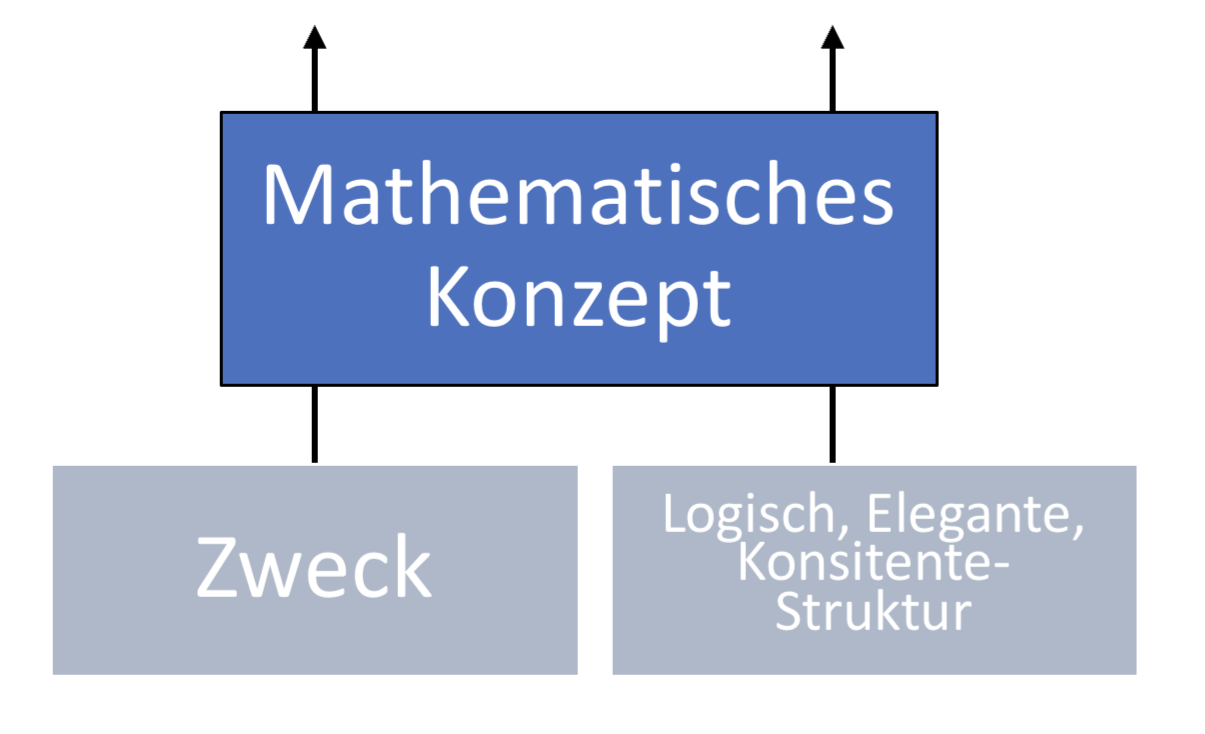
\includegraphics[width=0.3\linewidth]{attachment/chapter_8/Scc013}
\end{figure}

Beispiel \textit{Wahrscheinlichkeitsraum}. Dieser dient dem Zweck, später mit Zufallsvariablen arbeiten zu können und das Chaos realer Phänomen zu bändigen. Dies bildet den Zweck ab. Der Aufbau ist jedoch nach dem Treiber: \textit{Logisches, elegantes und konsistente Struktur} konzipiert.\\

Eine Herausforderung ist, dass der Zweck eines mathematischen Konzepts sich manchmal erst am Ende ergibt, weshalb der Aufbau sich manchmal erst ganz am Ende erschließt.
